\noindent Một khối băng hình bán cầu có bán kính $R$ và chiết suất $n$ nằm trên một mặt bàn ấm và được đun nóng từ từ. Nhiệt lượng do bàn truyền cho khối băng tỉ lệ với diện tích tiếp xúc giữa chúng. Biết rằng khối băng sẽ nóng chảy hoàn toàn sau thời gian $T_0$. Trong suốt quá trình, một chùm laser được chiếu vào khối băng. Chùm tia được chiếu theo phương vuông góc với bàn và cách trục đối xứng của băng một đoạn $\dfrac{R}{2}$ như hình 4.1.\\
\begin{figure}[h]
  \centering
  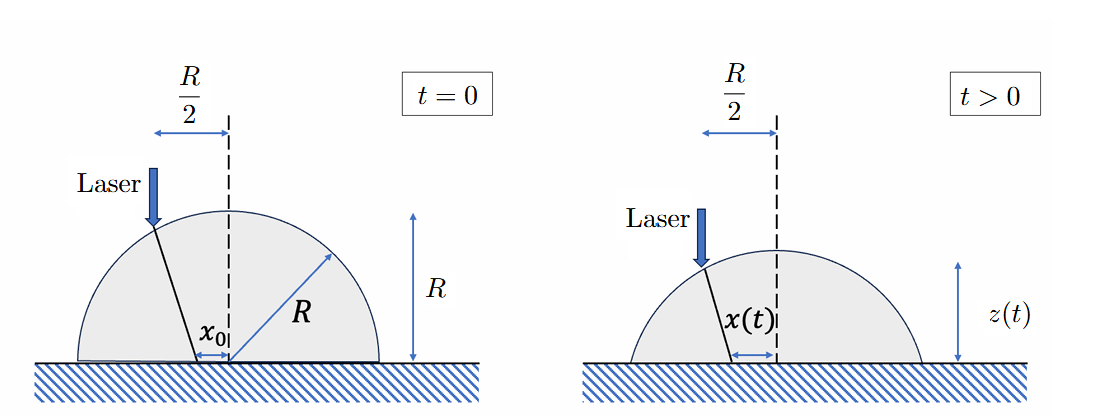
\includegraphics[width=1\textwidth]{Figures/Problems/Fig 4.1.png}
  \begin{center}
    \figurename{ 4.1}
  \end{center}
\end{figure}

\indent Giả sử nhiệt độ của khối băng và không khí bao quanh nó là $0^\circ$ trong suốt quá trình đun nóng. Chùm laser không truyền năng lượng cho khối băng. Toàn bộ lượng nước hình thành do sự nóng chảy đều chảy xuống bàn và khối băng không di chuyển trong suốt quá trình.
\begin{enumerate}
  \item Xác định vị trí $x_0$ mà tia laser chạm bàn tại thời điểm $t=0$ theo $n$ và $R$.
  \item Xác định độ cao của khối băng $z(t)$ tại thời điểm $t$ theo $R$ và $T_0$.
  \item Xác định vị trí $x(t)$ mà tia laser chạm bàn tại thời điểm $t\geqslant0$ theo $n, R, T_0$ và $t$.
\end{enumerate}